\documentclass[11pt]{article}
\usepackage[margin=0.9in]{geometry}
\usepackage{amsmath,booktabs,graphicx,enumitem,hyperref}
\hypersetup{colorlinks=true,urlcolor=blue,linkcolor=blue}
\setlength{\parindent}{0pt}
\setlength{\parskip}{0.6em}
\clubpenalty=10000
\widowpenalty=10000
\setlist{nosep,leftmargin=*}
\title{Learning to collect evidence against difficult targets}
\author{Results of the finite learning pilot}
\date{17 November 2026}
\begin{document}
\maketitle

Selecting difficult target interactions improved the information collected in
these small examples. Learning a distribution for proposing those targets added
little beyond proposing targets uniformly and keeping the hardest candidate.
Both approaches also handled an irreversible choice by balancing two competing
information needs. A positive residual error was the correct outcome in that
example.

The study completed all 72 registered runs: three environments, six paired
random seeds, and four methods. The independent replay found no missing runs or
failed checks. This report describes a finite learning experiment; the selected
paper has not been changed.

\section{The question and the learning procedure}

A \emph{collector} is the policy whose acquired record we evaluate. A
\emph{target} is another interaction we would like to reproduce from that
record. A \emph{decoder} randomly transforms the collected record into a
simulated target record. The same decoder must work in every possible world.
The simulation error measures the largest discrepancy between the simulated
and actual target distributions across those worlds. Each discrepancy is half
the sum of the absolute probability differences, the total variation distance.
Optimizing the decoder gives the best error the collected record can support
for that target.

The learned procedure keeps an archive of targets, beginning with a target that
reads the left bit twice. The collector and a separate decoder for each archived
target train together to reduce the largest fitted simulation error. A
generator then proposes four new candidates, and fresh decoder fitting estimates
how difficult each candidate is for the current collector. The hardest candidate
joins the archive. The collector trains against the enlarged archive before the
next proposal round. Keeping earlier targets makes lost capabilities continue
to affect the loss; the procedure does not require every target error to improve
at every update.

There are five proposal rounds. The generator learns three action distributions:
one for the initial action and one for each possible first observation.
These distributions propose a target that chooses the second action based on
the first observation. Generator updates use candidate errors as a heuristic
training signal. Those updates have no claim to
be an unbiased gradient of the complete search objective. The collector and
decoders use gradients of their finite empirical distribution losses.

Three controls separate the components. \emph{Uniform + random} proposes
candidates uniformly and retains a random candidate, independently of the
candidate scores. \emph{Uniform + hardest} uses the same uniform proposals but
retains the candidate with largest fitted error. \emph{All targets} trains
against every target from the beginning. The three candidate-search methods
have matching sampling, candidate-fitting and collector-update budgets; the
learned generator adds computation. The all-target method fits more decoders
and is an additional diagnostic.

\section{Environments, access, and evaluation}

Each environment has two hidden bits, with all four bit pairs possible. An
action reads left, reads right, or requests an independent fair coin. The
collector and every target receive two action--observation pairs. In
\emph{compatible readings}, either bit can be read exactly at either step. In
\emph{irreversible choice}, only the first action can yield information and the
second observation is always zero. In \emph{noisy readings}, each requested bit
is independently reported correctly with probability $0.85$.

Training receives 4,096 reset episodes from each labelled world, using uniform
random actions, and estimates a response table from these samples. The learner
uses those empirical tables. World labels group samples for the worst-world
loss, but neither the collector nor any decoder receives the world label.
Evaluation uses only a fresh two-step record from the frozen collector; the
training episodes are not part of that record. These are strong training access
assumptions, particularly for an environment whose evaluated interaction is
irreversible.

An independent evaluation uses the true response laws after training has
finished. A linear program computes the best decoder for each of the 27
deterministic two-step targets, and another optimization finds the smallest
possible largest-target error among all two-step stochastic collectors. Neither
calculation supplies updates or target-selection scores to the learner.

The collector parameterization keeps every action probability at least $0.005$.
The principal reference imposes the same restriction. For compatible readings,
removing that restriction reduces the optimum from $0.00748125$ to zero. For
irreversible choice, the unrestricted optimum is $1/4$: reading left or right
with equal probability leaves error $1/4$ on each bit target. The corresponding
restricted optimum is $0.25125$. For noisy readings, the unrestricted and
restricted numerical optima are approximately $0.077609$ and $0.077996$.

\section{Results and their interpretation}

Table~\ref{tab:final} reports the final collector's largest error across all 27
targets, after optimizing a decoder separately for each target. These values
measure information acquired by the collector, independently of whether the
learned decoders extract all that information.

\begin{table}[ht]
\centering
\small
\begin{tabular}{lrrr}
\toprule
Method & Compatible & Irreversible & Noisy \\
\midrule
Learned proposals + hardest & 0.007483 & 0.251362 & 0.094117 \\
Uniform proposals + hardest & 0.007485 & 0.251432 & 0.096168 \\
Uniform proposals + random & 0.008080 & 0.291801 & 0.110418 \\
All targets (extra decoder work) & 0.007489 & 0.251701 & 0.087863 \\
\midrule
Best with the same action restriction & 0.007481 & 0.251250 & 0.077996 \\
\bottomrule
\end{tabular}
\caption{Mean final worst-target simulation error over all six seeds; lower
is better. The last row is a numerical reference over all allowed collectors.
No seed was excluded. The small positive compatible-reading reference comes
from the imposed action randomization.}
\label{tab:final}
\end{table}

Both hardest-candidate methods rapidly approach the reference in the compatible
and irreversible environments (Figure~\ref{fig:curves}). Uniform random retention
usually reaches the same neighborhood, but can spend rounds adding targets
that expose no new information need. In the irreversible example, one of its
six runs never retains a target whose first action reads right. That run ends
at error $0.493930$; the other five end near $0.2514$. The missed right-bit
target explains most of the final mean difference.

\begin{figure}[ht]
\centering
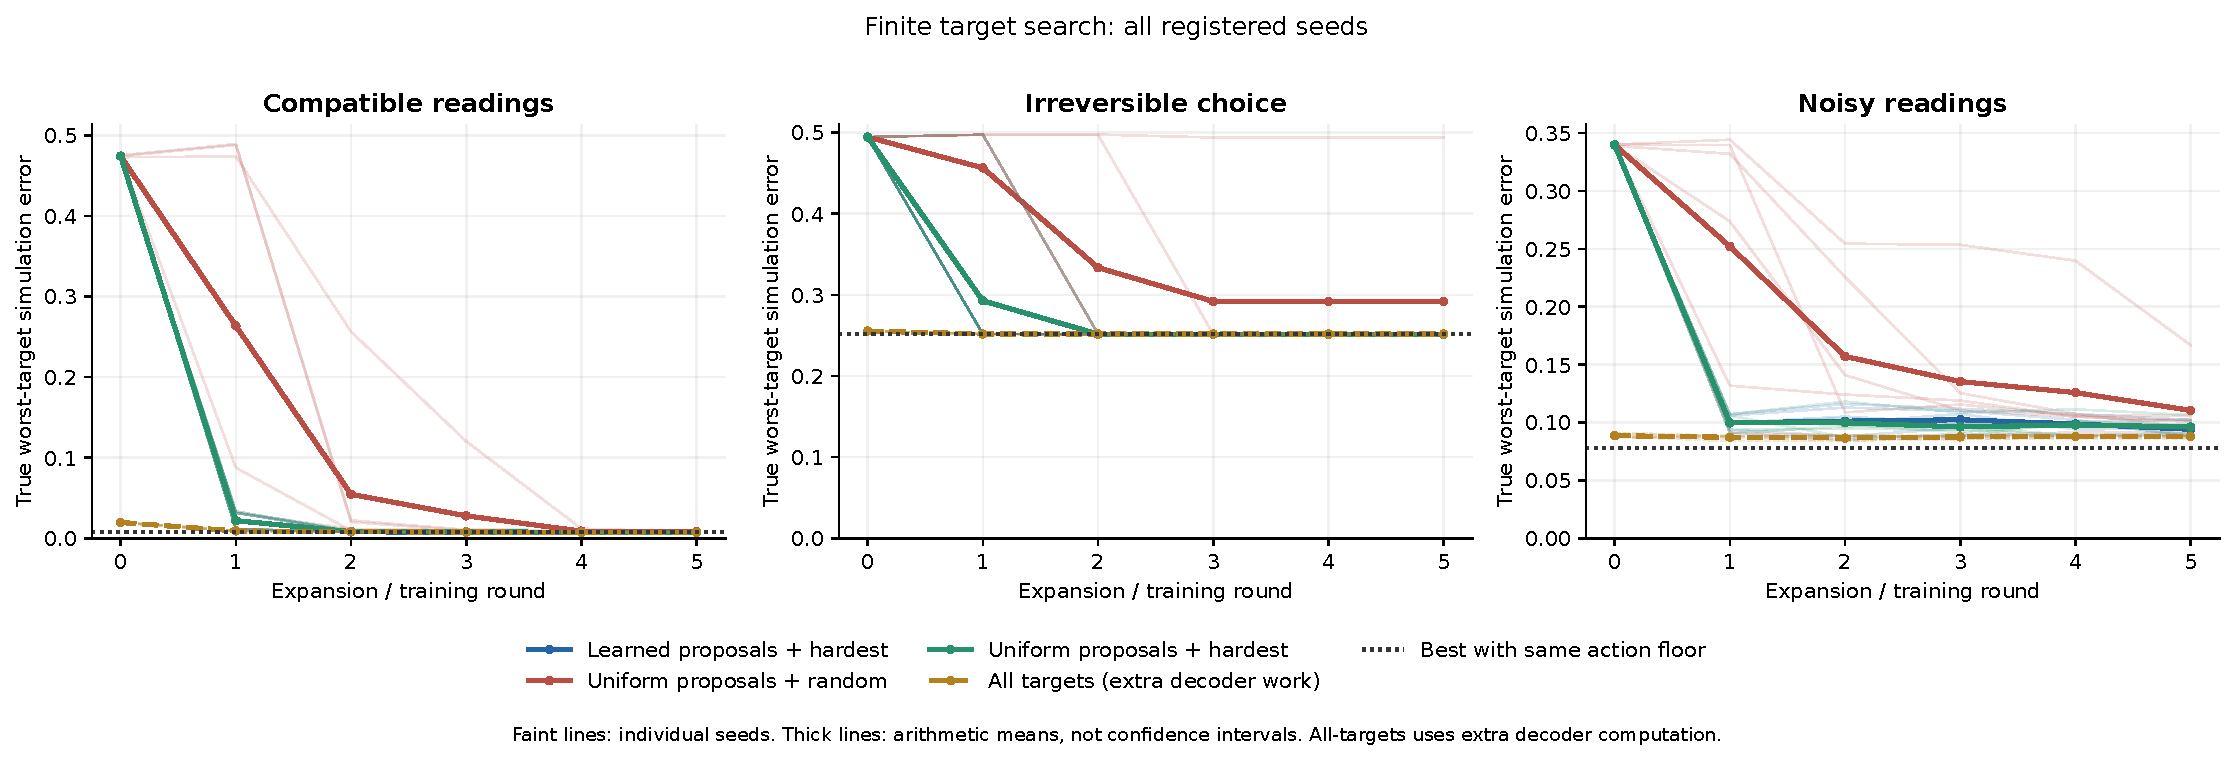
\includegraphics[width=\textwidth]{main/report/training_curves.pdf}
\caption{True simulation error after each training stage. Thick curves are
six-seed means, and faint curves retain every individual run. The dotted line
is the best error with the same action restriction. Stage zero follows training
on the initial archive; subsequent stages follow target additions. The
all-target diagnostic begins with all targets and uses extra decoder work at
every stage. The panels have different vertical ranges.}
\label{fig:curves}
\end{figure}

The noisy environment exposes a remaining limitation. Learned proposals reach
mean error $0.094117$, compared with $0.096168$ for uniform proposals with
hardest retention. The learned generator finishes better in four of six paired
seeds and worse in two. Averaging the five post-initialization stages instead
gives a slightly worse result for learned proposals: the paired mean difference
is $+0.001291$. Thus the final mean advantage does not establish a consistent
benefit from learning the proposal distribution. Training against all targets
reaches $0.087863$ but still exceeds the $0.077996$ reference. The six retained
targets, empirical-model error and optimization error all remain possible
contributors; this pilot does not isolate their causal contributions.

\section{The fitted decoders need a separate check}

A record can contain useful information even when its fitted decoder fails to
extract that information. We therefore compare each fitted decoder's error
with the best possible decoder error for the same record. We make that
comparison once in the empirical training model and again in the true model.
The empirical gap measures incomplete decoder fitting within the training
model. The true-model gap can also reflect the change from estimated to actual
response probabilities.

For learned proposals in the compatible environment, the mean largest empirical
fitting gap is $0.000250$, whereas the corresponding true-model gap is
$0.024821$. The collector's true optimal-decoder error is only $0.007483$.
Consequently the near-optimal collector should not be described as a complete
learned simulator. A particular fitted decoder can depend on accidental
world-dependent differences in the sampled fair-coin probabilities, even when
the best achievable information profile changes very little between the two
models. The saved diagnostics distinguish these quantities rather than assigning
the entire true-model gap to too few fitting steps.

The learned-proposal method selected no wholly world-independent target in its
90 additions. Its final probability of choosing the coin first averaged
$0.005000$, $0.005033$, and $0.006875$ in the compatible, irreversible, and noisy
environments, respectively. These observations support the intended distinction
between hard-to-simulate information and independent noise on these examples.
They do not guarantee that inaccurate fitted decoders could never make a noise
target look difficult.

\section{Checks, scope, and the next useful question}

Independent replay checked all 72 runs and 432 saved checkpoints, regenerated
all 18 sampled datasets, replayed 1,080 candidate-decoder scores, and checked the
six reference policies. A separate dense linear-program implementation
recomputed 15,228 target errors. The largest discrepancy outside the saved
sparse-program numerical interval was $1.98\times10^{-9}$, below the declared
comparison tolerance $2\times10^{-8}$. These are floating-point numerical
checks, not interval-arithmetic or Lean proofs. Source hashes, paired budgets,
random-selection independence and separation of training from true-model
evaluation also passed.

The pilot shows that a concrete finite search-and-training procedure can find
missing capabilities and accommodate tradeoffs. The present evidence favors
keeping the simple uniform-proposals/hardest-retention control central to any
follow-up. A larger target space would make learning the proposal distribution
a more substantive test, and separate checks would still be needed to determine
whether the fitted decoders transfer from the empirical model to the true law.

The procedure minimizes a finite largest-error criterion. The paper's reference
score $J_w$ instead subtracts a positively weighted average of eventual target
errors from one, so every strict coordinate improvement matters. A maximum can
tie such an improvement, and
finite search supplies no stopping certificate for the eventual score. The
pilot therefore establishes neither a numerical approximation guarantee for
$J_w$, complete exploration, nor performance on new world classes. The
\href{EXPLAINER.pdf}{pre-implementation explainer} gives the motivating example
and the maximum-versus-supremum distinction. The complete numerical tables,
paired differences and diagnostics are in
\href{main/report/RESULTS.md}{the generated report};
\href{REPRODUCE.txt}{the reproduction instructions} and
\href{AUDIT.txt}{the independent audit} provide the execution details.
\end{document}
